\section{Design}\label{sec:design}
\renewcommand{\imgpath}{tex/design/imgs}
\vspace{1cm}

\subsection{Overview}


\begin{figure}[H]
\centering
\begin{tikzpicture}
\node (raw) [data] {Lobster image};
\node (extraction) [process, right of=raw, xshift=2cm] {Keypoint extraction};
\node (creation) [process, right of=extraction, xshift=2cm] {Subgraph creation};
\node (subgraph) [data, right of=creation, xshift=2cm] {Lobster subgraphs};
\node (graphgrep) [process, right of=subgraph, xshift=2cm] {Subgraph matching};

\draw [arrow] (raw) -- (extraction);
\draw [arrow] (extraction) -- (creation);
\draw [arrow] (creation) -- (subgraph);
\draw [arrow] (subgraph) -- (graphgrep);

\end{tikzpicture}
\caption{Flow chart of the whole matching process from getting keypoints to creation of the lobster graphs.}
\end{figure}

\subsection{Annotation of dataset}
The dataset provided by \cite{lobster-thesis} was tagged with information on each image such as the lobster's sex, length of 

\imagefig{1\textwidth}{\imgpath/annotated.JPG}{Example of annotated lobster image with nodes and edges of the graph perfectly matched.}

\subsection{Keypoint detection}
First, to identify important parts from our lobster images, keypoints or areas of interest must be identified. OpenCV \cite{opencv} provides a host of different algorithms for feature detection such as Harris and Shi-Tomasi corner detectors and SIFT, SURF, ORB keypoint detectors \cite{opencv-tut1}. All these algorithms were tried and tested on a small subset of the dataset to see if any would provide both useful and consistent features that can be used. 

\begin{figure}[H]
%\centering
	\begin{subfigure}{0.45\textwidth}
	\includegraphics[width=\linewidth, scale=0.2, keepaspectratio]{\imgpath/img-harris.png}
	\caption{Harris corner detection}
	\end{subfigure}
	\hspace*{\fill}
	\begin{subfigure}{0.45\textwidth}
	\includegraphics[width=\linewidth, scale=0.2, keepaspectratio]{\imgpath/img-shi-tomasi.png}
	\caption{Shi-Tomasi corner detection}
	\end{subfigure}
	
	\vspace{0.5cm}
	
	\begin{subfigure}{0.45\textwidth}
	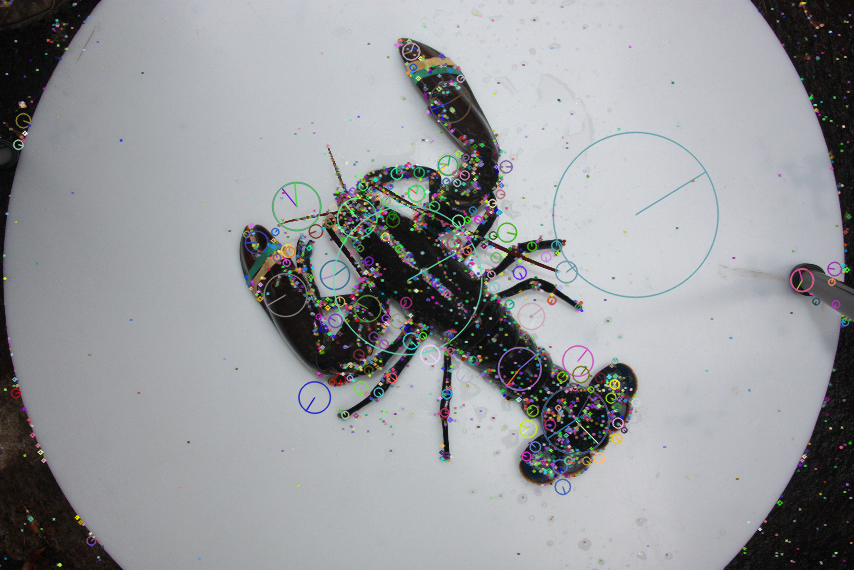
\includegraphics[width=\linewidth, keepaspectratio]{\imgpath/img-sift.png}
	\caption{SIFT keypoint detection}
	\end{subfigure}
	\hspace*{\fill}
	\begin{subfigure}{0.45\textwidth}
	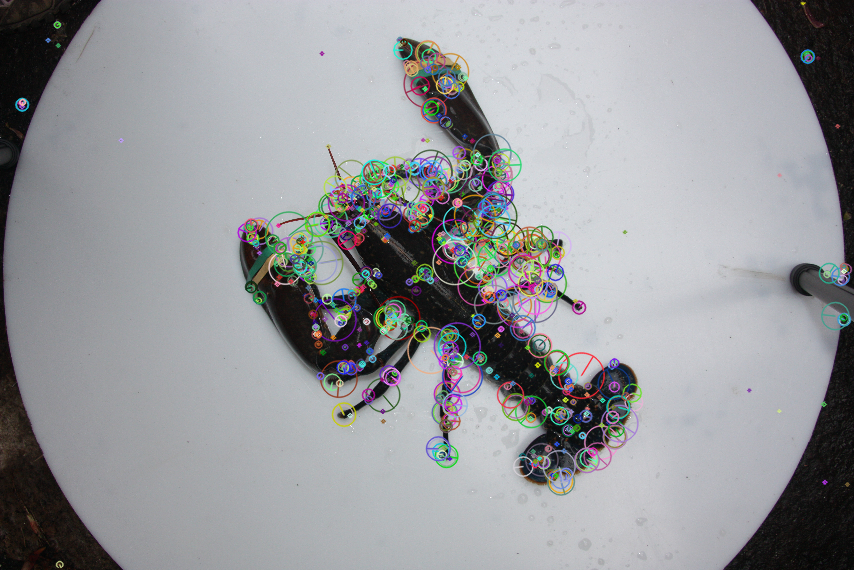
\includegraphics[width=\linewidth, keepaspectratio]{\imgpath/img-surf.png}
	\caption{SURF keypoint detection}
	\end{subfigure}
	
\caption{Comparison of different feature detection algorithms. The images have been scaled down after applying the detection to more clearly show the keypoints. Further comparison of the different detection algorithms on more images can be found in appendix \ref{apdx:cv-algos}}
\end{figure}
\begin{figure}[H]
%\centering
	\begin{subfigure}{0.45\textwidth}
	\includegraphics[width=\linewidth, scale=0.2, keepaspectratio]{\imgpath/img-harris2.png}
	\caption{Harris corner detection}
	\end{subfigure}
	\hspace*{\fill}
	\begin{subfigure}{0.45\textwidth}
	\includegraphics[width=\linewidth, scale=0.2, keepaspectratio]{\imgpath/img-shi-tomasi2.png}
	\caption{Shi-Tomasi corner detection}
	\end{subfigure}
	
	\vspace{0.5cm}
	
	\begin{subfigure}{0.45\textwidth}
	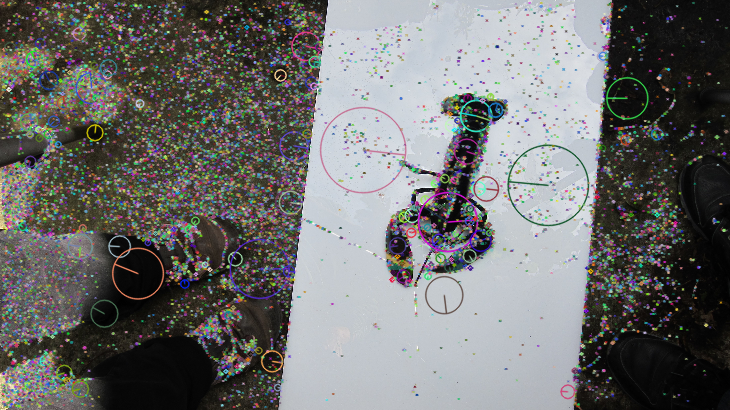
\includegraphics[width=\linewidth, keepaspectratio]{\imgpath/img-sift2.png}
	\caption{SIFT keypoint detection}
	\end{subfigure}
	\hspace*{\fill}
	\begin{subfigure}{0.45\textwidth}
	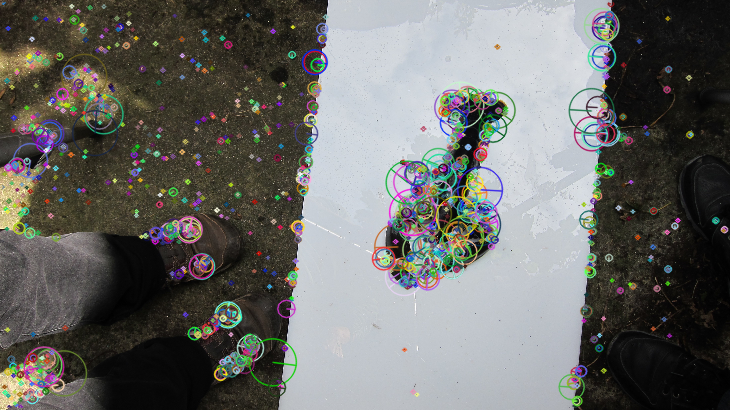
\includegraphics[width=\linewidth, keepaspectratio]{\imgpath/img-surf2.png}
	\caption{SURF keypoint detection}
	\end{subfigure}
	
\caption{Comparison of different feature detection algorithms on an image with more noise.}
\label{fig:kp-comparison-noise}
\end{figure}
\noindent
From visually seeing the effects of each algorithm, it can be seen that the corner detectors do not work very well for our purpose. The shape of the lobster is not fully detected reliably. For images with a noisier background, much of the background such as slabs with sharp contrasting corners are also detected, as shown in figure \ref{fig:kp-comparison-noise}. Furthermore, although corner detectors have applications in image matching \cite{corner-detection}, our goal from feature detection is to be able to extract graph like objects or features to apply graph matching on and so corner detection is unsuitable as we are not looking to match the different images to each other directly. 

The keypoint detectors are able to provide better results for our objective, as we can see keypoints of important body parts being identified, such as the body, tail and claws. These keypoints are further able to be consistently identified from multiple images, showing that use of these algorithms are promising for automatically detecting the various parts of the lobster for construction of a graph. There is still a lot of noise in the detected keypoints, but we shall see later in section \ref{sec:kp-filter} that different methods can be applied to filter out unwanted keypoints. It is also non-trivial to create a graph from an outline of corners to represent the shape of a lobster, whereas the keypoints naturally translate well as nodes of a graph, with edges connecting them to form the shape and pose of a lobster. Because of these reasons, the keypoint detection algorithms in SIFT, SURF and ORB were further investigated while the corner detectors were discarded.

\begin{figure}[H]
\centering
TODO  fig of keypoint detector algorithm comparison
\caption{Comparison of different keypoint detection algorithms on multiple lobster images. See comparison of more images in appendix \ref{apdx:cv-algos}}
\end{figure}
\noindent

Between the different keypoint detection algorithms, SIFT was chosen as it gave the most consistent results and the kind of useful keypoints that are needed. TODO


\subsection{Keypoint filtering}\label{sec:kp-filter}
From just running a SIFT detector on the lobster images, it can be seen that there are a lot of small keypoints that are unimportant for our purposes. There are also many keypoints around the lobster that we would like to filter out, as we want all our keypoints to be on the lobster. Initially, the classic vision approach for feature matching using the keypoint descriptors \cite{sift} was tried, but the results obtained were surprisingly poor. Because of this, a more novel approach was taken for filtering. The small keypoints are filtered out by specifying an octave where all keypoints coming from that octave or above are kept. Finally, remaining keypoints that are not on the lobster are filtered with a colour histogram method where the colour histograms of the keypoints are compared and any below a certain difference threshold are filtered away.

\subsubsection{SIFT descriptors}
In computer vision, keypoint descriptors obtained from detectors like SIFT and SURF are often used for feature matching \cite{cv-matching}. Lowe's paper \cite{sift} on the SIFT detector states that keypoints descriptors are highly distinctive, allowing a single feature to be correctly matching with good probability in a large database of features. This is exactly what we want, as we wish to extract the different features of a lobster (tail, claws, head). The only difference is we do not have a dataset of the lobsters, but not of dataset of individual lobster parts. 
\n
Because we do not have a dataset for individual parts, it made more sense to do the opposite of matching. Instead of using the distance between descriptors to match a detected keypoint with a known keypoint, the distance can be used as filter out keypoints that do not match closely to known ones. This distance can then be used as a threshold to filter more or less keypoints away. 
\n
As a test, the descriptor for the important body keypoint was taken from one image and calculated. The descriptor was then matched to the closest other keypoints on another image to see if the body could be identified again. 

\begin{figure}[H]
\centering
TODO keypoint descriptor matching other image
\caption{The image on the left shows the keypoint that the descriptor was calculated from and the image on the right is the closest TODO matched keypoints to that descriptor.}
\label{fig:kp-descriptor}
\end{figure}
\noindent
Figure \ref{fig:kp-descriptor} shows that the use of keypoint descriptors as a means of matching or filtering was not very reliable. TODO
\n
As the traditional method of descriptors proved unreliable for our means, a slightly more novel method was needed to filter out keypoints. (TODO sentance wording)

\subsubsection{Octave filtering}
The method of filtering by the actual size of the keypoints was first looked at before looking at octaves. It was found to be less robust and less general than using octave levels. There are a few issues involved in using size of the keypoint for filter, namely how to choose a suitable threshold. The size threshold must be constant across all images, otherwise the method will not be able to generalise to unseen images. The size of the keypoints is directly related to the size of the original image, so any size filter threshold must be calculated based on the size of the image. This is not an issue, as a constant size threshold can be relative to the size of the image. However, with different sizes of lobsters, an aggressive threshold may remove important keypoints that we wanted to keep. Conversely a more conservative threshold would not remove enough keypoints and cause a large combinatorial explosion, a problem explained later in section \ref{sec:probabilistic-model} that we wish to avoid. This makes it difficult to set a good threshold as it would have to be arbitrarily defined and based solely on manual inspection of the images and keypoints sizes of the dataset. Furthermore, this seems to be quite a crude method TODO. 

Octaves in SIFT are created by continually blurring an image. The idea behind this is to emulate looking at the image from different distances to get a varied set of keypoints. This means different features may be found at different octave levels. The high resolution of the images in our dataset causes many small keypoints to be found in the first few octave levels. These keypoints show many details that are irrelevant as we are concerned with the overall pose and size of the lobster.

\begin{figure}[H]
	\begin{subfigure}{0.5\textwidth}
	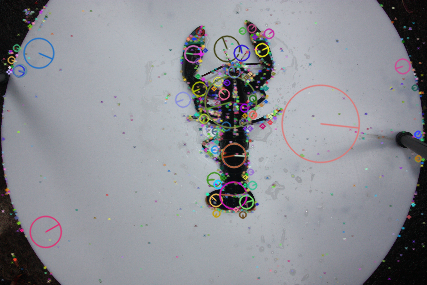
\includegraphics[width=\linewidth, keepaspectratio]{\imgpath/sift-raw.png}
	\caption{Before octave filtering}
	\end{subfigure}
	\hspace*{\fill}
	\begin{subfigure}{0.5\textwidth}
	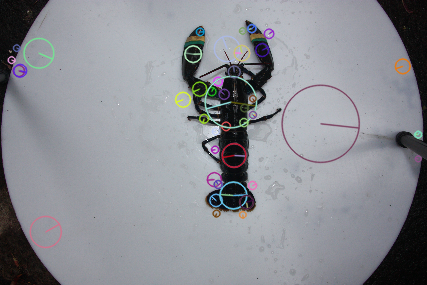
\includegraphics[width=\linewidth, keepaspectratio]{\imgpath/sift-octave.png}
	\caption{After octave filtering}
	\end{subfigure}
\caption{Before and after applying a filter on keypoints based on the octave level the keypoints were found in.}
\end{figure}
\noindent
From this observation, we can apply a filter on all keypoints found below a certain octave level so that we are only left with the larger keypoints that capture the features we are looking for. A filter for all keypoints found below octave level 3 was used. This octave level threshold is highly dependent on the size and resolution of the original image. An image with lower size and resolution may need a lower threshold or none at all (TODO reason). 


\subsubsection{Colour histogram filtering}
After applying the octave filter, there still remains some noisy keypoints we want to remove. Most notably are the keypoints found on the white background of the images. There have been studies \cite{color-histogram} \cite{color-filter} that show applying a colour filter to eliminate unwanted feature points can be quite effective, especially if the background is very different from the target of the image. Following from this, colour histograms of each keypoints were calculated and compared to a set of pre-defined histograms. The difference between the histograms was compared and only keypoints whose different is above a certain threshold are kept. 

\begin{figure}[H]
	\begin{subfigure}{0.5\textwidth}
	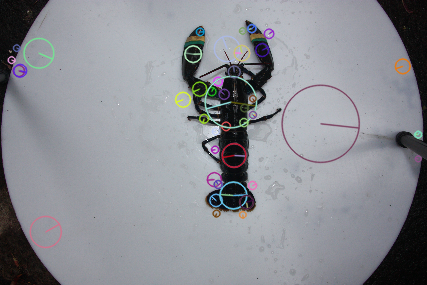
\includegraphics[width=\linewidth, keepaspectratio]{\imgpath/sift-octave.png}
	\caption{Octave filtering}
	\end{subfigure}
	\hspace*{\fill}
	\begin{subfigure}{0.5\textwidth}
	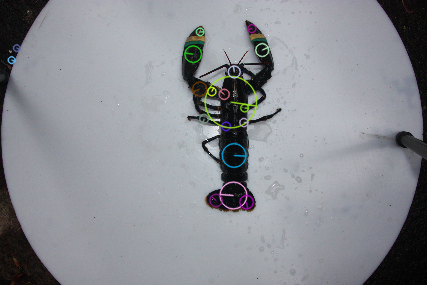
\includegraphics[width=\linewidth, keepaspectratio]{\imgpath/sift-histogram.png}
	\caption{Octave + colour histogram filtering}
	\end{subfigure}
\caption{Difference between applying only octave filtering and applying both octave and colour histogram filtering.}
\end{figure}
\noindent
The pre-defined histograms TODO

\subsection{Graph creation}

\subsubsection{Probabilistic model}\label{sec:probabilistic-model}


\subsection{Graph matching}

\subsubsection{Subgraph matching}

\subsubsection{Subgraph rebuilding}
